\documentclass{article}
\usepackage{indentfirst}


% Package imports
\usepackage{graphicx}  % For including images
\usepackage{amsmath}   % For mathematical formulas
\usepackage{amssymb}   % For math symbols
\usepackage{hyperref}  % For hyperlinks
\usepackage{booktabs}  % For better tables
\usepackage{multirow}  % For merging table cells
\usepackage{cite}      % For optimized citations
\usepackage{multicol}  
\usepackage{setspace}  % 用于调整行距
\usepackage{newtxtext}  % 设置 Times New Roman 字体
\usepackage{array}
\usepackage{pgfplots}
\usepackage{pgfplotstable}
\pgfplotsset{compat=1.18}
% Page layout
\usepackage[a4paper, margin=1in]{geometry}

% Hyperlink colors
\hypersetup{
    colorlinks=true,
    linkcolor=blue,
    citecolor=green,
    urlcolor=blue,
}


% Title and author information
\title{Lab 2: Branch Prediction}
\author{
  Peiyu Liu
}
\date{\today}


\begin{document}


\maketitle

\section{Introduction}
In this project, we delve into the design of branch predictors (BPs) in computer systems. Using the gem5 simulator, we evaluate the prediction accuracy of various BPs and develop our own customized branch predictors. Experimental results show that the perceptron predictor outperforms the Simple and Local predictors and is comparable to the BiMode and Tournament predictors.

\section{Experiment Setup}
To ensure a fair evaluation of the performance of different BPs, we ran the two benchmark programs provided in the course—spfa and shellsort—under identical CPU (O3CPU) and memory (DDR4) settings, with the only variable being the type of BPs integrated with the CPU. A brief summary of prediction strategies used by the BPs in this project is listed in Table \ref{table1}.

\begin{table}[h!]
\centering
\renewcommand{\arraystretch}{1.5}
\begin{tabular}{|>{\centering\arraybackslash}p{4cm}|>{\centering\arraybackslash}p{6cm}|>{\centering\arraybackslash}p{4cm}|}
\hline
\textbf{BP type} & \textbf{Strategy} & \textbf{Built-in / Customized} \\ 
\hline
LocalBP & Table of 2-bit counters& Built-in \\ 
\hline
BiModeBP & Choose between two direction predictors& Built-in \\ 
\hline
TournamentBP & Choose between global or local predictions& Built-in \\ 
\hline
SimpleBP & Always taken & Customized \\ 
\hline
PerceptronBP & A single-layer perceptron & Customized \\ 
\hline
\end{tabular}
\caption{Branch Predictor Strategies}
\label{table1}
\end{table}

As shown in Table \ref{table1}, We developed two customized branch predictors, SimpleBP and PerceptronBP, using the gem5 simulator. The SimpleBP employs an \textit{always-taken} strategy, consistently predicting branches as \textit{taken}, Meanwhile, the PerceptronBP is a reproduction of the approach described in the paper of \href{https://www.cs.utexas.edu/~lin/papers/hpca01.pdf}{Jiménez \textit{et al}.} In Section 4, the paper will be detailed summarized from three perspectives (motivations, challenges and designs).

To fully exploit the performance potential of the perceptron predictor, no hardware budget limitations are imposed. In the experiments, the prediction table is configured with ${2^{13}}$ entries (to better eliminate \textit{aliasing}), each corresponding to a perceptron containing 37 weights. With a history length ${h = 36}$ (since one of the weights serves as the bias), each weight is represented using 7 bits. This bit-width selection is informed by the presence of the threshold ${\theta= \lfloor 1.93h+14 \rfloor}$ (see Section \ref{4}). Therefore, storing all perceptrons requires approximately ${2^{18}}$ bytes.

\section{Results}
Table \ref{table2} presents the metrics used to evaluate the overall performance of various branch predictors on the benchmark programs. For conciseness, our analysis emphasizes the prediction accuracy of \textbf{conditional branches}, as these constitute the majority of branch instructions within the benchmark workloads. To minimize execution time, the maximum number of executed instructions is capped at $2\times10^8$,  a constraint that does not compromise the accuracy of the results.

\begin{table}[h!]
\centering
\renewcommand{\arraystretch}{1.5}
\begin{tabular}{|l|cc|cc|}
\hline
\multirow{2}{*}{\textbf{BP type}} & \multicolumn{2}{c|}{\textbf{Accuracy}} & \multicolumn{2}{c|}{\textbf{IPC}} \\ 
\cline{2-5}
 & \textbf{shellsort} & \textbf{spfa} & \textbf{shellsort} & \textbf{spfa} \\ 
\hline
LocalBP & 0.8025& 0.7776& 0.0431& 0.0487\\
BiModeBP & 0.8571& 0.7891& 0.0454& \textbf{0.0495}\\
TournamentBP & 0.8570& \textbf{0.7893}& 0.0454& 0.0494\\
SimpleBP& 0.4339& 0.5519& 0.0312& 0.0404\\
PerceptronBP& \textbf{0.8611}& 0.7885& \textbf{0.0456}& \textbf{0.0495}\\
\hline
\end{tabular}
\caption{Prediction Accuracy and IPC of Different BPs}
\label{table2}
\end{table}

Figure \ref{figure1} visualizes the statistical data presented in Table \ref{table2}. It is evident that the reproduced perceptron branch predictor (BP) outperforms both the SimpleBP and LocalBP, while demonstrating performance comparable to that of the BiMode BP and Tournament BP, thus meeting the project requirements. Additionally, the figure reveals a general trend: higher prediction accuracy correlates with an increase in instructions per cycle (IPC). This relationship is intuitive, as improved prediction accuracy reduces the frequency of pipeline stalls, thereby enhancing overall performance.

\begin{figure}[h!]
    \centering
    % 第一幅图：Accuracy
    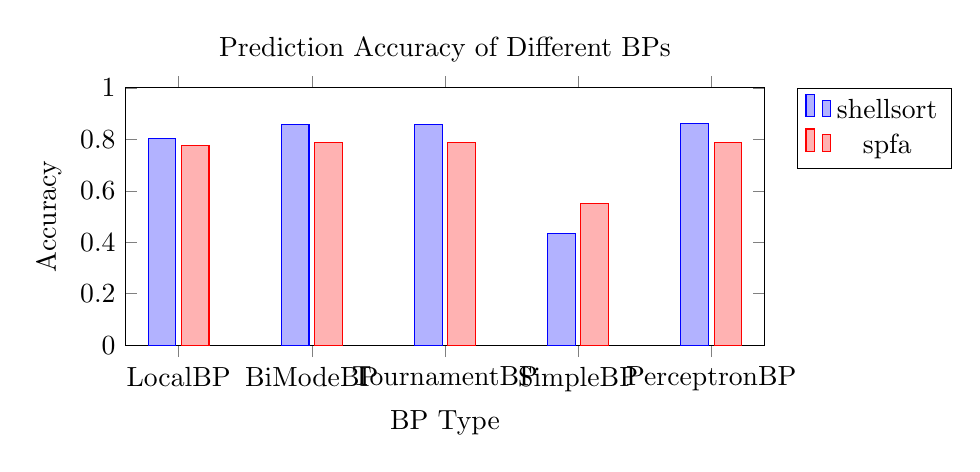
\begin{tikzpicture}
    \begin{axis}[
        width=0.8\textwidth,
        height=0.4\textwidth,
        bar width=10pt,
        symbolic x coords={LocalBP, BiModeBP, TournamentBP, SimpleBP, PerceptronBP},
        xtick=data,
        xlabel={BP Type},
        ylabel={Accuracy},
        title={Prediction Accuracy of Different BPs},
        ymin=0, ymax=1,
        legend style={at={(1.05,1)}, anchor=north west},
        ybar
    ]
    \addplot coordinates {(LocalBP,0.8025) (BiModeBP,0.8571) (TournamentBP,0.8570) (SimpleBP,0.4339) (PerceptronBP,0.8611)};
    \addplot coordinates {(LocalBP,0.7776) (BiModeBP,0.7891) (TournamentBP,0.7893) (SimpleBP,0.5519) (PerceptronBP,0.7885)};
    \legend{shellsort, spfa}
    \end{axis}
    \end{tikzpicture}

    \vspace{1cm}

    % 第二幅图：IPC
    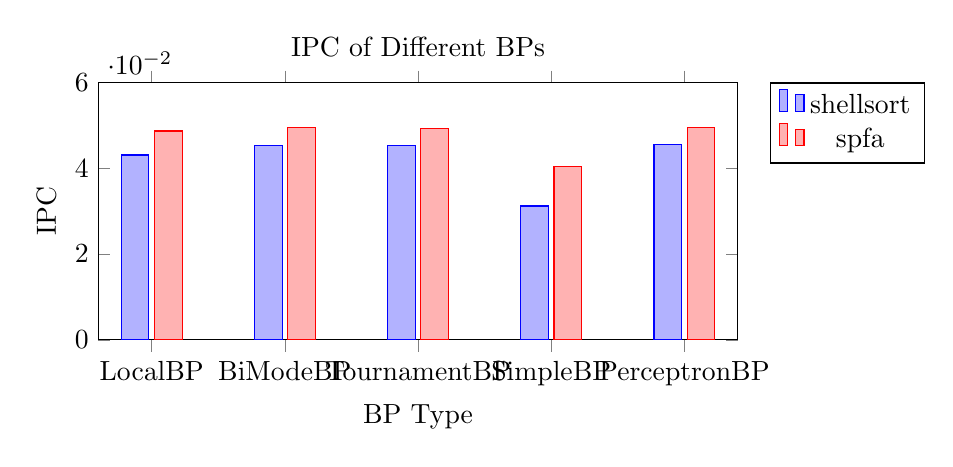
\begin{tikzpicture}
    \begin{axis}[
        width=0.8\textwidth,
        height=0.4\textwidth,
        bar width=10pt,
        symbolic x coords={LocalBP, BiModeBP, TournamentBP, SimpleBP, PerceptronBP},
        xtick=data,
        xlabel={BP Type},
        ylabel={IPC},
        title={IPC of Different BPs},
        ymin=0, ymax=0.06,
        legend style={at={(1.05,1)}, anchor=north west},
        ybar
    ]
    \addplot coordinates {(LocalBP,0.0431) (BiModeBP,0.0454) (TournamentBP,0.0454) (SimpleBP,0.0312) (PerceptronBP,0.0456)};
    \addplot coordinates {(LocalBP,0.0487) (BiModeBP,0.0495) (TournamentBP,0.0493) (SimpleBP,0.0404) (PerceptronBP,0.0495)};
    \legend{shellsort, spfa}
    \end{axis}
    \end{tikzpicture}
    \caption{Visualization of Prediction Accuracy and IPC}
    \label{figure1}
\end{figure}

\section{Paper Summary: Perceptron Predictor}\label{4}
The paper introduces a novel approach to dynamic branch prediction by employing one of the simplest neural networks, the perceptron, as an alternative to the widely used saturating counters. In contrast to saturating counters, the perceptron predictor efficiently utilizes a longer history length within the same hardware budget, as it allows hardware resources to scale\textbf{ linearly} with the increase in history length. Given the enhanced capacity to leverage more information, it is unsurprising that this method demonstrates superior performance compared to traditional techniques. However, an inherent limitation of the perceptron predictor lies in its ability to effectively predict only\textit{ linearly separable branches}. Fortunately, many branching behaviors in typical programs exhibit linear separability. Moreover, this limitation can be mitigated by developing a hybrid branch predictor, which combines the perceptron predictor with other methods.

\subsection{Challenges of Conventional Approaches}
\subsubsection{Limited history length}\label{Section 4.1.1}
Enhancing the prediction accuracy of BPs is critical to improving CPU performance, and these predictions depend on historical information, with longer histories generally resulting in higher accuracy. However, conventional methods relying on saturating counters restrict the amount of historical data that can be utilized. In these systems, the pattern history table (PHT) stores a counter for each branch (ideally), indexed by a global history register (GHR). To ensure the PHT remains within a manageable size, the length of the GHR must be limited, following a \textbf{logarithmic} relationship with the amount of counters.

\subsubsection{\textit{Aliasing}}
Due to hardware constraints on history length, traditional methods primarily focus on mitigating \textit{aliasing} to improve prediction accuracy. \textit{Aliasing} occurs when two unrelated branches interfere with each other by utilizing the same prediction resources, leading to inaccurate predictions. However, given the limitations of hardware resources, it is challenging to eliminate \textit{aliasing} entirely. Conventional approaches attempt to reduce this interference by designing effective hash functions to compute the index of the PHT for each branch, minimizing the overlap in resource usage.

\subsection{Motivations of the New Approach}

\subsubsection{Utilizing Longer History Records}
As discussed in Section \ref{Section 4.1.1}, the use of saturating counters prevents conventional branch predictors from leveraging long history lengths effectively. This limitation motivates the exploration of alternative components, such as perceptrons, which can store longer histories with fewer hardware constraints, thereby improving the prediction process.

\subsubsection{Focusing on Prediction Accuracy}
While traditional methods focus heavily on mitigating \textit{aliasing}, the limited history length may pose a more significant barrier to enhancing prediction accuracy. Thus, the new approach prioritizes improving accuracy by utilizing more comprehensive historical information, rather than solely minimizing aliasing.

\subsubsection{Extracting More Information from Predictor States}
Another key motivation may lie in the interpretability of perceptrons, which store much more states compared to traditional 2-bit counters. By analyzing the weights of a specific perceptron, it becomes possible to infer correlations between the target branch and other recent branches. This additional information is effectively provided at no extra cost and can be leveraged to gain deeper insights into branch behavior, further enhancing the analysis and optimization of branch predictors.

\subsection{Designs of Perceptron Predictor}
\subsubsection{General Principles}
Generally speaking, perceptron predictor replaces the saturating counters in the PHT (e.g., 2-bit counters) of conventional BPs. The steps to make a prediction are summarized as follows:

1.  The branch address is hashed to produce an index $i$ into the PHT.

2.  The $i^{th}$ perceptron (composed of weights) is fetched into a vector register $P_{0...n}$. 

3.  Compute $y$, the dot product of $P$ and the global history register.

4.  The branch is predicted not taken when $y$ is negative, or taken otherwise.

5.  Once the actual outcome of the branch becomes known, weights in $P$ are updated.


6.  $P$ is written back to the $i^{th}$ entry in the PHT.

\subsubsection{Training Strategy}
The actual outcome of branches serves as feedback for the perceptron. The weights corresponding to the history branches that align with the outcome should be increased and those don't align with the outcome should be reduced. This adaptive adjustment ensures that the perceptron learns from past behavior, improving its accuracy over time by reinforcing useful patterns and diminishing the influence of misleading correlations.

\subsubsection{Implementation}
Several major challenges arise when implementing the perceptron predictor in hardware.

The first challenge is the computational complexity of the perceptron. To address this, the weights are restricted to integer values, eliminating the need for floating-point arithmetic and thus reducing computational overhead.

Another important problem is \textit{aliasing}, which occurs when multiple branches interfere by sharing the same prediction resources. This issue can be alleviated by increasing the size of BHT. However, under limited hardware resources, we must keep the size of each perceptron (i.e., the weights) small to increase the size of BHT.

In the referenced paper, the authors introduced a threshold $\theta$ to limit the range of weights. They found that the optimal threshold follows the formula:
$$\theta = \lfloor 1.93h + 14\rfloor$$
where $h$ is the history length. By confining the output $y$ within the range of $[-\theta, \theta]$, all weights remain within the range, ensuring no overflow occurs. As a result, each weight can be represented in $1+\lfloor log_2 \theta \rfloor$ bits. This compact representation allows every perceptron in the PHT to be stored more efficiently, optimizing memory usage and hardware space.
\end{document}

